\chapter{Background} \label{chap:background}

\section{Deep Learning}
\subsection{Motivations}
Deep learning has recently been highly successful in machine learning across a variety of application domains, including computer vision, natural language processing, and big data analysis, among others. For example, deep learning methods have consistently outperformed traditional methods for object recognition and detection in the ISLVRC Computer Vision Competition since 2012 \cite{ILSVRC15}. However, deep learning’s high accuracy comes at the expense of high computational and memory requirements for both the training and inference phases of deep learning. Training a deep learning model is space and computationally expensive due to millions of parameters that need to be iteratively refined over multiple time epochs. Inference is computationally expensive due to the potentially high dimensionality of the input data (e.g., a high-resolution image) and millions of computations that need to be performed on the input data.

\subsection{Definitions}
As described in \cite{Goodfellow-et-al-2016}, the modern term “deep learning” goes beyond the neuroscientific perspective engineering applications on the current breed of machine learning models. It appeals to a more general principle of learning \textit{multiple levels of composition}, which can be applied in machine learning frameworks that are not necessarily neurally inspired.
A deep learning prediction algorithm, consists of a number of layers, as shown in Fig. \ref{fig:dnn}.

\begin{figure}
	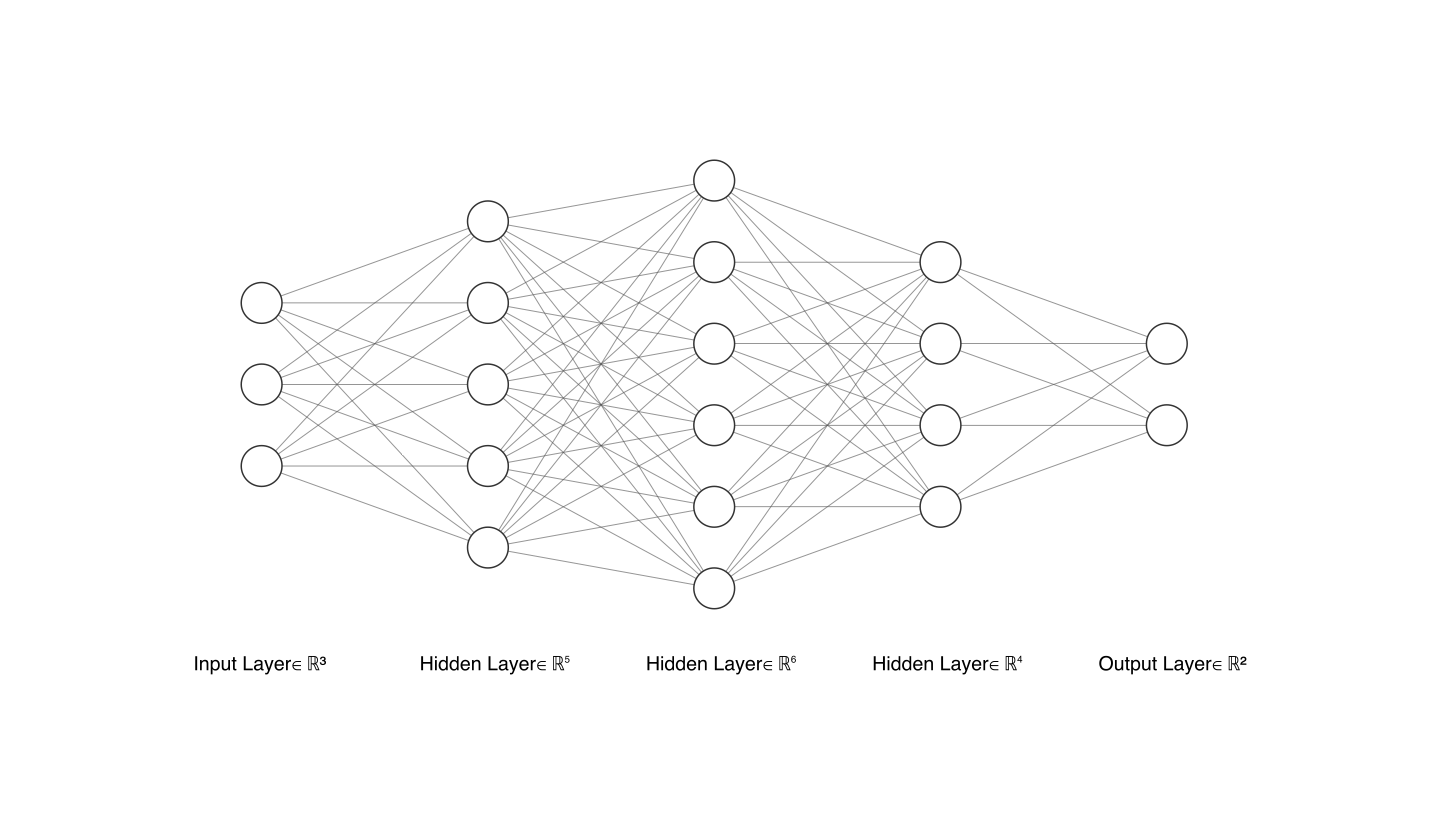
\includegraphics[width=\textwidth]{images/nn.png}
	\caption[DNN example]{DNN example with image classification}
	\label{fig:dnn}
\end{figure}

In deep learning \textit{inference}, the input data pass through the node's layers in sequence, and each layer performs matrix multiplications on the data. The output of a layer is usually the input to the subsequent layer. After data are processed by the final (fully connected) layer, the output is either a feature or a classification value. When the model contains many layers in sequence, the neural network is known as a deep neural network (DNN). When the matrix multiplications include convolutional filter operations, the model is named convolutional neural networks (CNNs), which is common for image and video processing contexts. There are also DNNs designed especially for time series prediction; these are called recurrent neural networks (RNNs), which have loops in their layer connections to keep state and enable predictions on sequential inputs.

In deep learning \textit{training}, the computation proceeds in reverse order. Given the ground-truth training labels, multiple passes are made over the layers to optimize the parameters of each layer of matrix multiplications, starting from the final layer and ending with the first layer. The algorithm used is typically stochastic gradient descent (SGD).  In each pass, a randomly small subset of N input data ("mini-batch") from the training data set, is selected and used to update the gradients in the direction that minimizes the training loss (where the training loss is defined as the difference between the predictions and the ground truth). One pass through the entire training data set is called a training epoch \cite{ruder2016overview}.

There are some considerations to take into account: the first is that there are a large number of parameters in the matrix multiplications, resulting in many computations being performed and thus the latency issues that we see on end devices. The second is that there are many choices (hyper-parameters) on how to design the DNN models (e.g., the number of parameters per layer, and the number of layers), which makes the model design more of an art than a science. Different DNN design decisions result in tradeoffs between system metrics; for example, a DNN with higher accuracy likely requires more memory to store all the model parameters and will have higher latency because of all the matrix multiplications being performed. On the other hand, a DNN model with fewer parameters will likely execute more quickly and use less computational resources and energy, but it may not have sufficient accuracy to meet the application's requirements.


\subsection{Performance Measurement}
How can we evaluate the performance of a neural network?
Deep learning can be used to perform both supervised learning and unsupervised learning. The metrics of success depend on the particular application domain where deep learning is being applied. For example, in object detection, the accuracy may be measured by the mean average precision (mAP) \cite{ILSVRC15}, which measures how well the predicted object location overlaps with the ground-truth location, averaged across multiple categories of objects. In machine translation, the accuracy can be measured by the bilingual evaluation understudy score metric \cite{10.3115/1073083.1073135}, which compares a candidate translation with several groundtruth reference translations. 
Other general system performance metrics not specific to the application include throughput, latency, and energy. These metrics are summarized in Table \ref{tab:NN-Perfomance-Metrics}.
Designing a good DNN model or selecting the right DNN model for a given application is challenging due to the large number of hyperparameter decisions.

\begin{table}[htbp]
	\centering
	\begin{tabular}{|l||c|} 
	\hline 
	 Metric & Unit	\\
	\hline
	Latency  &	s	\\
	Energy	& mW, J	\\
	Concurrent Requests Served	&	\#  \\
	Network Bandwidth	& Mbps			  \\
	Accuracy & Application Specific		\\
	\hline
	\end{tabular}
	\caption{Neural Network Perfomance Metrics\label{tab:NN-Perfomance-Metrics}}
\end{table}

Machine learning research typically focuses on accuracy metrics, and their system performance results are often reported from powerful server testbeds equipped with GPUs. For example, Huang et al. \cite{huang2016speedaccuracy} compared the speed and accuracy tradeoffs when running on a high-end gaming GPU (NVIDIA Titan X). The YOLO DNN model \cite{YOLO9000}, which is designed for real-time performance, provides timing measurements on the same server GPU.
Specifically targeting mobile devices, Lu et al. \cite{CNN-mobile} provided the measurements for a number of popular DNN models on mobile CPUs and GPUs (Nvidia TK1 and TX1). Ran et al.\cite{Ran-DNN-edge-video-analisys} further explored the accuracy-latency tradeoffs on mobile devices by measuring how reducing the dimensionality of the input size reduces the overall accuracy and latency. DNN models designed specifically for mobile devices, such as MobileNets \cite{howard2017mobilenets}, report system performance in terms of a number of multiply–add operations, which could be used to estimate latency characteristics and other metrics on different mobile hardware, based on the processing capabilities of the hardware.
Once the system performance is understood, the application developer can choose the right model. 


\subsection{Frameworks}
Several open-source software libraries are publicly available for deep learning inference and training on end devices and edge servers. Google’s TensorFlow \cite{tensorflow2015-whitepaper}, released in 2015, is an interface for expressing machine learning algorithms and an implementation for executing such algorithms on heterogeneous distributed systems. Tensorflow's computation workflow is modeled as a directed graph and utilizes a placement algorithm to distribute computation tasks based on the estimated or measured execution time and communication time \cite{abadi2016tensorflow}. The placement algorithm uses a greedy approach that places a computation task on the node that is expected to complete the computation the soonest. Tensorflow can run on edge devices, such as Raspberry Pi and smartphones. TensorFlow Lite was proposed in the late 2017 \cite{tensorflowlite}, which is an optimized version of Tensorflow for mobile and embedded devices, with mobile GPU support added in early 2019. 
Tensorflow Lite only provides on-device inference abilities, not training, and achieves low latency by compressing a pre-trained DNN model.
Caffe \cite{Caffe} is another deep learning framework, originally developed by Jia, with the current version, Caffe2, maintained by Facebook. It seeks to provide an easy and straightforward way for deep learning with a focus on mobile devices, including smartphones and Raspberry Pis. PyTorch \cite{NEURIPS2019_9015} is another deep learning platform developed by Facebook, with its main goal differing from Caffe2 in which it focuses on the integration of research proto- types to production development. Actually Facebook is working on the merge of Caffe2 and PyTorch frameworks.
GPUs are an important key element in efficient DNN inference and training. NVIDIA provides GPU software libraries to make use of NVIDIA GPUs, such as CUDA \cite{CUDA} for general GPU processing and cuDNN \cite{cuDNN} which is targeted toward deep learning. While such libraries are useful for training DNN models on a desktop server, cuDNN and CUDA are not widely available on current mobile devices such as smartphones. To utilize smartphone GPUs, Android devel- opers can currently make use of Tensorflow Lite, which provides experimental GPU capabilities. To experiment with edge devices other than smartphones, researchers can turn to edge-specific development kits, such as the Nvidia Jetson TX2 development kit for experimenting with edge computing (e.g., as used in [33]), with Nvidia-provided SDKs used to program the devices.



\subsection{Challenges}
Because of the required competences and effort to choose the best neural network and the best parameters that better fit the application of interest, there has also been much recent interest in automated machine learning, which uses artificial intelligence to choose which DNN model to run and tune the hyperparameters. 
For example, Tan et al. \cite{tan2018mnasnet} and Taylor et al. \cite{taylor2018adaptive} proposed using reinforcement learning and traditional machine learning, respectively, to choose the right hyperparameters for mobile devices, which is useful in edge scenarios.

%%%%%%%%%%%%%%%%%%%%%%%%%%%%%%%%%%%%

\section{Edge Computing}

\section{Docker}

\section{Kubernetes}


\clearpage
\thispagestyle{empty}